%%%%%%%%%%%%%%%%%
%Nome: Nicolas P. Lane
%Data: 13/10/2015
%D�vidas ou contribui��es: nicolaspeterlane@hotmail.com
%%%%%%%%%%%%%%%%%

\NeedsTeXFormat{LaTeX2e}
%-----------------------------------------------------------
\documentclass[a4paper,12pt]{monografia}
\usepackage{amsmath, amsthm, amsfonts, amssymb}
\usepackage[english, brazilian]{babel}
\usepackage[titletoc]{appendix}
\usepackage[latin1]{inputenc}
\usepackage[mathcal]{eucal}
\usepackage[alf]{abntcite}
\usepackage{subfigure}
\usepackage{url}
\usepackage{isoaccent}
\usepackage{textcase}
\usepackage{multirow}
\usepackage{latexsym}
\usepackage{graphicx}
\usepackage{listings}
\usepackage{acronym}
\usepackage{bm}
\usepackage{comment}
\usepackage{float}

\usepackage{stmaryrd}

\usepackage{pgf,tikz}
\usepackage{tkz-graph}  
\usetikzlibrary{shapes.geometric}%   

\usepackage{csquotes}

\lstset{basicstyle=\tiny, language=C++}
\makeindex
%-----------------------------------------------------------Come�a documento
\begin{document}
%----------------- T�tulo e Dados do Autor -----------------
\titulo{An�lise e solu��o de vulnerabilidades em ambiente LAMP baseada em experimenta��o com Kali Linux}
\autor{Aurelio Grott, Gabriel Dominico, Victor Lucas de M. Mafra}
\nome{}
\ultimonome{}

%---------- Informe o Curso e Grau -----
\bacharelado \curso{Ci\^encia da Computa\c{c}\~ao} \mes{Junho} \ano{2016} 
\data{\today} % data da aprova��o
\cidade{Joinville}

%----------Informa��es sobre a Institu��o -----------------
\instituicao{Universidade do Estado de Santa Catarina}
\sigla{UDESC} \unidadeacademica{Centro de Ci\^encias Tecnol\'ogicas}

%------Nomes do Orientador, 1o. Examinador e 2o. Examinador-
\orientador{Charles Christian Miers}
\examinadorum{Charles Christian Miers}
\examinadordois{Charles Christian Miers}
%\examinadorquatro{Nome do Examinador 4}

%--------- T�tulos do Orientador 1o. e 2o. Examinadores ----
\ttorientador{Doutor}
\ttexaminadorum{Doutor}
\ttexaminadordois{Doutor}
%\ttexaminadorquatro{T�tulo do Examinador 4}

\maketitle
%---------------------- AGRADECIMENTO --------------
\agradecimento{Agradecimentos}



\newpage
%---------------------- EP�GRAFE --------------
\begin{epigrafe}

  ``We must know - we will know!''\\ - David Hilbert

\end{epigrafe}
%--------Digite aqui o seu resumo em Portugu�s--------------
\resumo{Resumo}
Este trabalho visa a compreensão da %chamada de arquivo resumo.tex

\noindent Palavras-chaves: 
%-----------Digite aqui o seu resumo em Ingl�s--------------
\resumo{Abstract}
\ac{SDN} is a new technology which gives the network administrator greater power over his
network. Such control is given through the separation between the control plane and the
data plane, which characterizes an \ac{SDN}. 
%
In this paper it is conceptualized several key points relative to \ac{SDN}, such as \textit{OpenFlow}
and the \ac{SDN} planes. In the following section it is described the networking simulation tool
\textit{Mininet} folowwing by the description of two benchmarks that will be used with the 
objective of data collection for later analisys.
%
Since the hardwares that supports \ac{SDN} are relatively new, their costs is very often
prohibitively high for a small research group or an independent researcher, so that the
use of simulators becomes indispensable for the technological and scientific development in
the field.
%
This paper has as its major objective to do an comparative between the transferering of
medium sized data in a Mininet simulated environment and a traditional networking model 
(i.e.\ coupled Data Plane and Control plane).
%
%
%Assistive Technology (AT) is a knowledge field used to identify resources in order to provide or
%expand skills of people with disabilities, mobility disability or reduced mobility. 
%This work initially presents a bibliography research about people with disabilities, specifically
%people who have Cerebral Palsy (CP) followed by an applied research in order to specify the
%requirements and project for a Extended Alternative Communication software solution. 
%Based on the set of people with CP, this work addresses specifically the people who have limited
%locomotor skills in addition to speech difficulties. 
%The alternative solution software specification presented in this work allows these people to
%communicate with their therapists in order to stimulate their cognition. 
%This paper is organized as follows: context, research results related to people with disabilities;
%AT initiatives and their taxonomies, the specification of the problem that is addressed in the
%work; and specification of the proposal suggested by the author. 
%However, the AT initiatives tend to have some regionalism directed related to local demands. 
%Thus, this work also includes interactions with the Associa��o dos Deficientes de Joinville (ADEJ)
%in order to identify this regional context and the Grupo Assitiva of the Santa Catarina State
%University (UDESC).
     %chamada de arquivo abstract.tex

\noindent Keywords:
%-----------------------------------------------------------

\listoffigures       %gera p�gina com lista de figuras a partir de todas as entradas feitas no documento

% lista de abrevia��es
\listoftables        %gera p�gina com lista de tabelas a partir de todas as entradas feitas no documento
\chapter*{Lista de Siglas e Abreviaturas}
\addcontentsline{toc}{chapter}{Lista de Siglas e Abreviaturas}
\begin{acronym}

\acro{ASP}[ASP]{Apache Software Foundation}
\acro{BD}[BD]{Banco de dados}
\acro{CGI}[CGI]{Common Gateway Interface}
\acro{CVE}[CVE]{Common Vulnerabilities and Exposures}
\acro{DNS}[DNS]{Domain Name System}
\acro{DoS}[DoS]{Denial of Service}
\acro{GNU}[GNU]{Gnu Not Unix}
\acro{GPL}[GPL]{General Public License}
\acro{HTTP}[HTTP]{HyperText Transfer Protocol}
\acro{LAMP}[LAMP]{Linux Apache MySQL PHP}
\acro{PHP}[PHP]{Hypertext Preprocessor}
\acro{SGBD}[SGBD]{Sistema de Gerenciamento de Banco de Dados}
\acro{SMTP}[SMTP]{Simple Mail Transfer Protocol}
\acro{SQL}[SQL]{Structured Query Language}
\acro{UDESC}[UDESC]{Universidade do Estado de Santa Catarina}
\begin{comment}
\acro{CLI}[CLI]{Command Line Interface}
\acro{CPU}[CPU]{Central Processing Unit}
\acro{DPCF}[DPCF]{Data Plane Control Function}
\acro{IETF}[IETF]{Internet Engineering Task Force}
\acro{IO}[I/O]{Input/Output}
\acro{LSD}[LSD]{Link State Database}
\acro{NFS}[NFS]{Network File System}
\acro{ONF}[ONF]{Open Networking Fundation}
\acro{OSPF}[OSPF]{Open Shortest Path First}
\acro{PRNG}[PRNG]{Pseudo-Random Number Generator}
\acro{QOS}[QOS]{Quality of Service}
\acro{RAM}[RAM]{Random Access Memory}
\acro{SDN}[SDN]{Software Defined Network}
\acro{SNMP}[SNMP]{Simple Network Management Protocol}
\end{comment}

\end{acronym}
    %chamada de arquivo acronimos.tex

%----Sum�rio, lista de figura e de tabela ------------
\tableofcontents      %gera p�gina com sum�rio a partir de todas as entradas feitas no documento

\newpage

%--------------In�cio do Conte�do---------------------------
\pagestyle{ruledheader} %estilo abnt2
\chapter{Introdu��o}
\label{cap:introducao}

Atualmente, com a grande explos�o de crescimento da Internet e do \textit{Cloud Computing}, as redes de computadores
se tornaram cada vez mais complexas, demandando cada vez mais esfor�os para gerenci�-las. Com o objetivo de melhorar
e faciliar o gerenciamento de grandes redes, um novo paradigma de rede foi introduzido, o \textit{Software Defined
Network} (SDN). O \ac{SDN} caracteriza-se pela separa��o n�tida do \textit{Data Plane} do \textit{Control Plane}.
Tal separa��o permite que o administrador tenha o controle de sua rede atrav�s de uma camada de abstra��o, permitindo
distribuir e controlar os recursos de sua rede de um ponto logicamente centralizado sem ter que acessar individualmente
cada dispositivo de rede. O uso do \ac{SDN} deu ao administrador de redes a capacidade de alterar qualquer por��o da
rede assim que necess�rio, seja a altera��o uma prioriza��o, redirecionamento ou bloqueamento de pacotes em espec�fico.
Isto tornou-se essencial nos ambientes modernos de \textit{Cloud Computing} onde volumes in�ditos de informa��o est�o
dispon�veis.


Para que o uso do \ac{SDN} cres�a, al�m da divulga��o e acessibilidade, � necessario promover o desenvolvimento
cientifico e tecnol�gico. Atualmente existe uma organiza��o dedicada a promover o a promo��o e ado��o do \ac{SDN},
a \textit{Open Networking Foundation} (ONF). A ONF foi respons�vel por apresentar e desenvolver o \textit{OpenFlow},
protocolo que fornece uma abstra��o dos recursos de rede. O \textit{OpenFlow} � tido como a primeira padroniza��o
aberta de SDN e � considerada um elemento central no desenvolvimento.


O SDN � uma tecnologia relativamente nova no mercado, e isto se traduz em pre�os elevados, muitas vezes proibitivos
para universidades e outras institui��es que promovem o desenvolvimento cient�fico e tecnol�gico. Como alternativa
ao uso de \textit{Hardware} compativel com SDN, existe a possibilidade da utiliza��o de simuladores e emuladores
tais como o \textit{Mininet}. No entanto � preciso conhecer suas capacidades e validar seus resultados. Este trabalho
tem como objetivo comparar o desempenho fornececido pelo \textit{Mininet} com uma situa��o real de transfer�ncia de
arquivos de m�dio porte.


     %chamada de arquivo introducao.tex
\chapter{Conceitos}
\label{cap:conceitos}

\section{LAMP}
\label{sec:lamp}


\subsection{HIST�RICO}
\label{subsec:historico}


\subsection{APLICABILIDADE}
\label{subsec:aplicabilidade}


\section{FUNCIONAMENTO E COMPONENTES B�SICOS}
\label{sec:componentes}

\subsection{Linux}
\label{subsec:linux}

Linux poderia ser descrito como um sistema operacional similar a 
qualquer outro, como Windows e OS X. Por�m tem algo que o destaca dos demais, 
desde sua origem em 1991, e que � o motivo do sistema ter crescido e ganhado
uma grande for�a na computa��o, atualmente presente em lugares desde a bolsa
de valores de Nova York e supercomputadores  � telefones celulares e computadores
pessoais, o Linux � um software livre desenvolvido de maneira
colaborativa \cite{WhatI30:online}. Mais de 1.000 desenvolvedores
de pelo menos 100 diferentes companhias, contribu�ram para cada
vers�o do kernel sob a licensa \ac{GPL} que � baseada em quatro
liberdades \cite{Whati7:online}:

\begin{itemize}
 \item A liberdade de executar o programa como quiser, para qualquer prop�sito;
 \item A liberdade para estudar como o programa funciona, e alter�-lo para que ele execute como voc� queira. Ter acesso ao c�digo fonte � necess�rio para tal;
 \item A liberdade para redistribuir c�pias para ajudar o pr�ximo; e
 \item A liberdade para distribuir c�pias de suas vers�es modificadas para outros. Fazendo isso voc� concede � comunidade a chance de se beneficiarem de suas altera��es. Ter acesso ao c�digo fonte � necess�rio para tal.
\end{itemize}

Por esses motivos o Linux tem sido bem-sucedido, particularmente como plataforma de servidor: 
at� mesmo em organiza��es que confiam veemente em sistemas operacionais
comerciais como Microsoft Windows, o Linux aparece frequentemente em papeis infraestruturais, como em \textit{gateways} de \ac{SMTP} e servidores \ac{DNS}
devido a sua confian�a, seguran�a, baixo custo e a qualidade execepcional das aplica��es do servidor \cite{bauer2005linux}.

\subsection{Apache}
\label{subsec:apache}

Atuando como servidor \ac{HTTP} no sistema \ac{LAMP}, o Apache � o servidor \textit{web}
mais popular na Internet desde Abril de 1996 \cite{http:apache}.
O Apache � um projeto de c�digo livre (sob a licensa \ac{GPL}) da \ac{ASP}, o qual tem como 
objetivo manter um seguro, eficiente e extens�vel servidor que prov�
servi�os \ac{HTTP} de acordo com os padr�es \ac{HTTP} atuais.

\subsection{MySQL}
\label{subsec:mysql}

O \ac{BD} MySQL, foi projetado com base no mSQL, o qual tinha muitos problemas, como 
n�o ser r�pido e flex�vel o suficiente para o uso dos usu�rios, com isso a necessidade
de um novo \ac{BD} foi aumentando e com base nesse conceito foi desenvolvido o que
hoje conhecemos como MySQL, por isso � o \ac{BD} do servidor LAMP.

Um \ac{BD} pode ser definido como uma cole��o de dados. Por�m para conseguir acessar
os dados armazenados nesse sistema, teve-se a necessidade de criar algum tipo de gerenciador,
sendo o MySQL um dos mais usados. Algumas caracter�sticas \cite{MySQL69:online} desse sistema podem ser vistas abaixo:

\begin{itemize}
 \item \textbf{Banco de dados relacional:} a principal diferen�a desse tipo de \ac{BD} para os outros
 � que os dados s�o guardados em pequenas tabelas de uma forma que seu acesso seja da forma mais eficiente
 o poss�vel.
 \item \textbf{\textit{Open Source:}} esse termo corresponde que qualquer pessoa pode modificar o 
 \textit{software} do jeito que preferir, podendo ajust�-lo conforme a sua necessidade.
 \item \textbf{R�pido, confi�vel, escal�vel e f�cil de usar:} como foi criado para atender a grandes
 quantidades de dados de uma forma mais r�pida que seus concorrentes, foi apenas l�gico que se tornasse
 um dos mais r�pidos \ac{BD}. Portanto come�ou a ser utilizado em grande escala, consequentemente a 
 seguran�a foi aumentando juntamente com sua escalabilidade para atender a demanda de usu�rios. 
\end{itemize}

Contudo, mesmo com medidas de seguran�as sendo tomadas, precisamos ainda tomar algumas atitudes para 
dificultar que seu \ac{BD} seja acessado por pessoas n�o autorizadas, alguns m�todos b�sicos que 
ajudam a proteger s�o descritas abaixo \cite{MySQL10:online}:

\begin{itemize}
 \item N�o prover acesso a ningu�m para a tabela usu�rio do \ac{BD} MySQL.
 \item N�o guardar senhas sem algum tipo de fun��o \textit{hash} (algoritmo usado para transformar 
 sua senha para uma \textit{string} ileg�vel.
 \item Crie senhas ale�torias, por�m de f�cil memoriza��o.
 \item Invista em um \textit{firewall}, protegem pelo menos 50\% dos ataques feitos contra seu \textit{software}.
 \item Sempre criptografe os dados que precisam ser enviados pela internet.
\end{itemize}



\subsection{PHP}
\label{subsec:php}

O \ac{PHP} foi criado em 1994 por Rasmus Lerdof, o projeto inicial era um simples conjunto de \ac{CGI}s bin�rios escritos na linguagem de
programa��o C, usados para rastrear as visitas ao seu \textit{site}. Com o tempo, otimiza��es foram sendo feitas e funcionalidades adicionadas.
Sendo lan�ado em 1998, o \ac{PHP} 3.0 foi a primeira vers�o que cont�m tra�os do \ac{PHP} de hoje em dia, incluindo o suporte a programa��o orientada a
objeto. Por�m essa vers�o tinha muita dificuldade em processar aplica��es complexas, foi com base nessa premissa que foram lan�adas as vers�es 4.0
e 5.0 (Julho de 2004), principalmente para melhorar seu antecessor e acrescentar dezenas de novos recursos.

Usado principalmente para desenvolvimento \textit{web}, � um \textit{script open source} de uso geral. Podemos especificar em quais �reas os 
\textit{scripts} \ac{PHP} s�o mais utilizados \cite{PHP:O35:online}, como:
\begin{itemize}
 \item \textbf{Scripts no lado do servidor.} Podendo acessar os resultados do seu programa com um navegador web.
 \item \textbf{Scripts de linha de comando.} Executar os scripts sem um servidor ou navegador, apenas necessita de um interpretador PHP.
 \item \textbf{Escrever aplica��es desktop.} N�o � a melhor linguagem para se desenvolver aplica��es desktop, por�m para um programador experiente o PHP tem alguns recursos
 avan�ados que permitem escrever esse sistema.
\end{itemize}

Uma caracter�stica � a escalabilidade que o \ac{PHP} possui, podendo ser utilizado na maioria
dos sistemas operacionais e servidores \textit{web}. Com isso ele vem sendo aplicado cada
vez mais em servidores LAMP, por suas v�rias extens�es que facilitam a conectividade com diversos banco de dados.


\section{FUNDAMENTA��O DE ATAQUE E SOLU��ES}
\label{sec:fundamentos}

Testes de penetra��o de servidores \textit{web} n�o devem ser confundidos com ataques maliciosos. Apesar de possuirem rotinas 
parecidas, possuem objetivos distintos. Ataques maliciosos s�o realizados para roubar informa��es, causar indisponibilidade de servi�os
(\ac{DoS}) ou qualquer outro evento indesejado ao respons�vel pelo servidor. J� um teste de penetra��o consiste em um processo 
autorizado, programado e sistem�tico onde se faz uso de vulnerabilitades conhecidas para realizar tentativas de invas�o � um servidor,
rede ou conte�dos de aplica��es.

Testes de penetra��o podem ser executados de mais de uma maneira para propor mais de um ponto de vista sob a mesma organiza��o. 
Para tal, existem dois tipos de testes (n�o exclusivos) que podem ser conduzidos \cite{sans:2002}.

\begin{description}
      \item[Teste  interno de penetra��o] Realizado com o objetivo de identificar vulnerabilidades com acesso
      f�sico ou exposi��o a engenharia social. Servem para determinar quais vulnerabilidades existem no sistema interno, 
      acess�vel somente � pessoas autorizadas com acesso a rede interna da organiza��o.

      \item[Teste externo de penetra��o] Realizado com o objetivo de identificar vulnerabilidades presentes atrav�s de
      conex�es que foram estabelecidas atrav�s da conex�o entre a organiza��o e a Internet (atrav�s do \textit{firewall} ou \textit{gateway}).
\end{description}

\section{FRAMEWORKS E SOLU��ES PARA AN�LISE DE VULNERABILIDADES}
\label{sec:frameworks}

\section{NORMAS, RECOMENDA��ES E BOAS PR�TICAS PARA AN�LISE DE VULNERABILIDADES}
\label{sec:normas}


Vulnerabilidade pode ser definida como um erro no \textit{software} que permita ao \textit{hacker} ganhar acesso ao sistema ou a rede interna \cite{CVE-F22:online}. Primeiramente 
monitoramos com qual frequ�ncia determinada vulnerabilidade pode ocorrer, e o qu�o prejudicial � para o programa. Quando descobrimos alguma vulnerabilidade com os testes realizados,
podemos verificar em algum banco de dados de vulnerabilidades, sendo o \ac{CVE} uma boa fonte para conhecer um pouco mais sobre o problema encontrado. 

Temos tamb�m os chamados escaneadores de vulnerabilidade, os quais s�o \textit{softwares} que ajudam na identifica��o de poss�veis problemas que podem facilitar a corrup��o do 
sistema, identificando, como por exemplo: vers�es de \textit{softwares} desatualizadas, configura��es falhas. Segundo \cite{NIST:online}, esses escaneadores podem:

\begin{itemize}
 \item \textbf{Verificar pol�ticas de seguran�a.}
 \item \textbf{Prover informa��es sobre alvos para testes de penetra��o.}
 \item \textbf{Fornecer informa��es sobre como diminuir as vulnerabilidades descobertas.}
\end{itemize}

Contudo, mesmo com esses facilitadores, ainda temos alguns problemas a serem vencidos, como quando pequenos riscos de vulnerabilidade s�o analisados de uma forma isolada, por�m 
quando observados como um conjunto podem trazer um grande problema ao sistema, isso pode ser dito como uma das principais falhas desses escaneadores, pois conseguem apenas analisar 
amea�as ind�viduais e n�o em um escopo espec�fico.

Outro meio de se prevenir contra ataques pode ser feito com uma simples revis�o do c�digo fonte quando est� sendo implementado, n�o apenas no seu estado final. Tamb�m � vi�vel realizar 
testes unit�rios para verificar a consist�ncia presente no c�digo.


\begin{comment}

  EXEMPLO DE FIGURA

  \begin{figure}[!h]
  \centering
  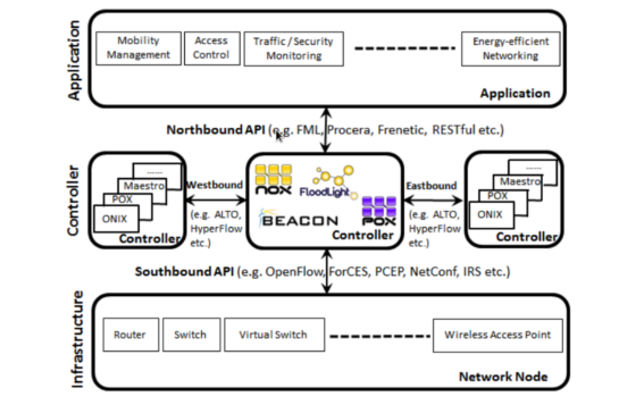
\includegraphics[scale=0.7]{sdnARCH.png}
  \caption{Diagrama da arquitetura de uma SDN.}
  \label{fig:sdnArch}
  \end{figure}

  EXEMPLO DE DESCRI��O DE ALTERNATIVAS

  \begin{description}
      \item[Maxinet] Baseado no \textit{Mininet}, possui o objetivo de superar as limita��es em rela��o ao
      n�mero de dispositivos de rede que podem ser simulados. Segundo o autor~\cite{maxinet}, o \textit{Maxinet} tem
      como prop�sito simular grandes redes de \textit{data-centers} e superar o desempenho do \textit{Mininet} atrav�s
      da utiliza��o de v�rios computadores trabalhando de forma distribu�da. O \textit{Maxinet} cont�m \textit{built-in} um
      gerador de trafego de rede, baseado em recentes an�lises de casos reais.

      \item[Mininet-Hifi] O \textit{Mininet-Hifi}~\cite{mininethifi} � um projeto com a finalidade de melhorar
      a reprodutibilidade de testes realizados no \textit{Mininet}. Implementado de forma semelhante, utilizando 
      \textit{containers}, o \textit{Mininet-Hifi} utiliza de recursos adicionais para melhorar a reprodutibilidade. 
  \end{description}

\end{comment}




\chapter{Conclus�o}

Conclus�o conclus�o conclus�o conclus�o conclus�o conclus�o conclus�o conclus�o conclus�o conclus�o conclus�o conclus�o conclus�o conclus�o
 conclus�o conclus�o conclus�o conclus�o conclus�o conclus�o conclus�o conclus�o conclus�o conclus�o conclus�o conclus�o conclus�o
  conclus�o conclus�o conclus�o conclus�o conclus�o conclus�o conclus�o conclus�o conclus�o conclus�o
   conclus�o conclus�o conclus�o conclus�o conclus�o conclus�o conclus�o conclus�o conclus�o conclus�o conclus�o conclus�o conclus�o conclus�o
    conclus�o conclus�o conclus�o conclus�o conclus�o conclus�o conclus�o conclus�o conclus�o conclus�o conclus�o conclus�o conclus�o conclus�o
     conclus�o conclus�o conclus�o conclus�o conclus�o conclus�o conclus�o conclus�o conclus�o conclus�o conclus�o conclus�o conclus�o conclus�o
      conclus�o conclus�o conclus�o conclus�o conclus�o conclus�o conclus�o conclus�o conclus�o conclus�o conclus�o conclus�o conclus�o conclus�o
 conclus�o conclus�o conclus�o conclus�o conclus�o conclus�o conclus�o conclus�o conclus�o conclus�o conclus�o conclus�o conclus�o conclus�o conclus�o
  conclus�o conclus�o conclus�o conclus�o conclus�o conclus�o conclus�o conclus�o conclus�o conclus�o conclus�o conclus�o conclus�o conclus�o conclus�o
  


      %chamada de arquivo capitulos.tex (desenvolvimento de seu TCC efetivamente)

%--------------Bibliografia e ap�ndices--------------------
\bibliographystyle{abnt-alf}
\bibliography{bibliografia}

		%chamada de arquivo anexo.tex
\appendix

\chapter{Exemplo num{\'e}rico da primeira contribui{\c{c}}{\~a}o}

Considerando como entrada ao algoritmo uma imagem em n{\'i}veis de cinza de dimens{\~o}es $1 \times 20$, representada na figura \ref{fig:entrada_exemplo_numerico}, observa-se a exist{\^e}ncia de dois m{\'a}ximos regionais: $50$ e $43$. Por meio destes m{\'a}ximos, {\'e} poss{\'i}vel encontrar suas $k$ maiores extin{\c c}{\~o}es. No exemplo adotado, ser{\'a} considerada a maior extin{\c c}{\~a}o de cada tipo de atributo crescente e ser{\~a}o apresentados os c{\'a}lculos baseados no atributo altura.

\begin{figure}[ht]
	\centering
	\caption{Imagem de entrada do exemplo.}
	\includegraphics[scale=1.0]{imagens/exemplo_numerico.png} \\
	Fonte: Imagem gerada pela autora.
    \label{fig:entrada_exemplo_numerico}
\end{figure}

A partir da imagem de entrada, portanto, {\'e} necess{\'a}rio encontrar o m{\'a}ximo regional com a maior extin{\c c}{\~a}o de altura. Analisando a figura \ref{fig:entrada_exemplo_numerico_extincao}, {\'e} determinada a maior extin{\c c}{\~a}o de altura no m{\'a}ximo $50$, este utilizado nos c{\'a}lculos para gera{\c c}{\~a}o da imagem simplificada. Assim, a partir das coordenadas deste m{\'a}ximo regional {\'e} calculado seu {\'i}ndice representativo a partir do intervalo de normaliza{\c c}{\~a}o escolhido. Este c{\'a}lculo {\'e} efetuado por meio de duas f{\'o}rmulas:

\begin{figure}[ht]
	\centering
	\caption{Extin{\c c}{\~o}es de altura.}
	\includegraphics[scale=1.0]{imagens/exemplo_numerico_extincao.png} \\
	Fonte: Imagem gerada pela autora.
    \label{fig:entrada_exemplo_numerico_extincao}
\end{figure}

\begin{equation}
	I = x_{c} \times nc + y_{c}
\end{equation}

\begin{equation}
	In = i \ (nl \times nc) \times Indice
\end{equation}

onde $x_{c}$ e $y_{c}$ representam, respectivamente, a linha e a coluna da coordenada do m{\'a}ximo de maior altura, $nl$ e $nc$ o n{\'u}mero de linhas e colunas da imagem de entrada, $i$ o n{\'u}mero de unidades do intervalo de normaliza{\c c}{\~a}o, e $I$ e $In$ os valores dos {\'i}ndices antes e ap{\'o}s a normaliza{\c c}{\~a}o, respectivamente. Assim, a partir do valor da coordenada ($0$, $4$) do m{\'a}ximo $50$ e considerando o intervalo de normaliza{\c c}{\~a}o de $0$ a $255$, {\'e} determinado um {\'i}ndice normalizado que o representar{\'a}:

\begin{equation}
	Indice = 0 \times 20 + 4 = 4
\end{equation}

\begin{equation}
	Indice\_normalizado = 255 \ (1 \times 20) \times 4 = 51
\end{equation}

Desta forma, $51$ {\'e} o valor do {\'i}ndice normalizado da maior extin{\c c}{\~a}o de altura da imagem de entrada. Este n{\'u}mero corresponde {\`a}primeira linha ({\'i}ndices do atributo altura) e coluna da imagem simplificada. O c{\'a}lculo dos {\'i}ndices normalizados {\'e} repetido para todos os atributos de valores de extin{\c c}{\~a}o, formando assim, para este exemplo, a imagem simplificada:

\begin{center}
$\left[
	\begin{array}{c}
		51 \\
		ind\_area \\
		ind\_volume \\
		ind\_altura\_caixa \\
		ind\_largura\_caixa \\
		ind\_nro\_descendentes \\
		ind\_altura\_topologica 
	\end{array} 
\right]$
\end{center}

sendo $ind\_area$, $ind\_volume$, $ind\_altura\_caixa$, $ind\_largura\_caixa$, $ind\_nro\_de$ $scendentes$ e $ind\_altura\_topologica$ os {\'i}ndices correspondentes {\`a} maior extin{\c c}{\~a}o de {\'a}rea, volume, altura e largura da caixa envolvente, n{\'u}mero de descendentes e altura topol{\'o}gica da sub-{\'a}rvore, respectivamente. Ap{\'o}s a gera{\c c}{\~a}o das imagens simplificadas para entradas e treinamentos, estas s{\~a}o aplicadas ao algoritmo do PCA para o reconhecimento.
	%chamada de arquivo apendice.tex
\end{document}
